\documentclass[crop,tikz]{standalone}
\usepackage{pgfplots}

% http://pgfplots.net/tikz/examples/bell-curve/
\pgfplotsset{compat=1.8}
\pgfmathdeclarefunction{gauss}{2}{\pgfmathparse{1/(sqrt(#2*2*pi))*exp(-((x-#1)^2)/(2*#2))}}
\pgfmathdeclarefunction{multigauss}{4}{\pgfmathparse{1/(sqrt(#2*2*pi))*exp(-((x-#1)^2)/(2*#2)) * 1/(sqrt(#4*2*pi))*exp(-((y-#3)^2)/(2*#4))}}

\pgfplotsset{colormap={whiteblack}{color(0cm)=(white); color(1cm)=(gray)}}

\usetikzlibrary{positioning,shapes,arrows}

\begin{document}
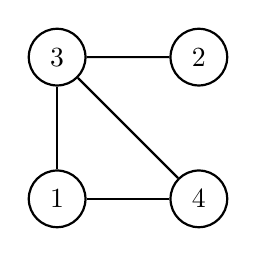
\begin{tikzpicture}
    [scale=.6,auto=left,every node/.style={draw, thick, circle, inner sep = 0pt, minimum width = 0.72cm}]
  \node (n1) at (1,1) {1};
  \node (n2) at (4,4) {2};
  \node (n3) at (1,4) {3};
  \node (n4) at (4,1) {4};

  \foreach \from/\to in {n1/n3, n1/n4, n2/n3, n3/n4}
    \draw (\from) edge[thick] (\to);
\end{tikzpicture}
\end{document}
